\documentclass{article}
\usepackage{graphicx}
\begin{document}

\title{Playing Random Playlist Report}
\author{SATTIRAJU R N S SAI SATWIK}
\maketitle

\section{Introduction}
In this report, we will discuss the implementation of a program that plays a random playlist using the VLC media player. The program utilizes the `os`, `vlc`, `numpy`, and `curses` modules to load audio tracks, shuffle them randomly, and provide key-based control for playback.


\section{Code Description}

The script performs the following steps:

\begin{enumerate}
  \item It loads all the audio tracks in the specified playlist directory.
  \item The audio tracks are shuffled randomly using the NumPy library.
  \item A VLC media player instance is created.
  \item The script initializes the curses module for text-based user interface.
  \item Each audio track is played in the shuffled order.
  \item The script waits for the track to finish playing or for user input.
  \item The user can press 'q' to stop playback, 'n' to play the next song randomly, 'p' to pause the song, or 'b' to play the previous song randomly.
  \item After all tracks have been played, the player is released and the curses module is cleaned up.
\end{enumerate}

\section{Usage}

To use the script, follow these steps:

\begin{enumerate}
  \item Ensure you have the necessary Python libraries installed (vlc, numpy, curses).
  \item Set the correct path to your playlist directory in the \texttt{playlist\_directory} variable.
  \item Execute the script.
\end{enumerate}



\begin{figure}[htbp]
  \centering
  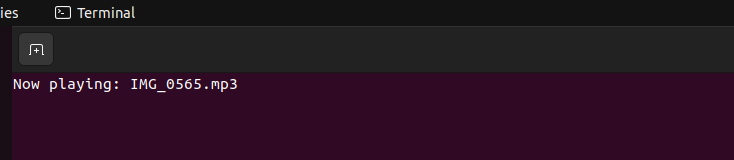
\includegraphics[width=0.6\textwidth]{Screenshot from 2023-05-18 18-05-33.png}
  \caption{This is how my console looks while compiling the code}
  \label{fig:example_image}
\end{figure}


\end{document}

